\section{Experiment \& Result} \label{section:experiment_result}

To prove our hypotheses, the authors test both the BoW systems with and without spatial rerank on the Oxford Building 5K Dataset \cite{oxbuilding}. This dataset was constructed by Philbin et al. in 2007 \cite{2}. It consists of 5,062 images of resolution $1024 \times 768$ belongs to 11 different Oxford buildings. Images for each building are collected from Flickr by searching using text queries. In figure \ref{fig:oxbuilding}, some samples from the dataset are shown. Along with the dataset, there are also 55 queries along with their ground-truth, 5 for each landmark, as shown in figure \ref{fig:oxbuilding_query}. The reason why the authors use this dataset is because of its popularity, it is used by many previous works in this field. Thus, we can easily compare our systems with those previous works.

\begin{figure}
    \centering
    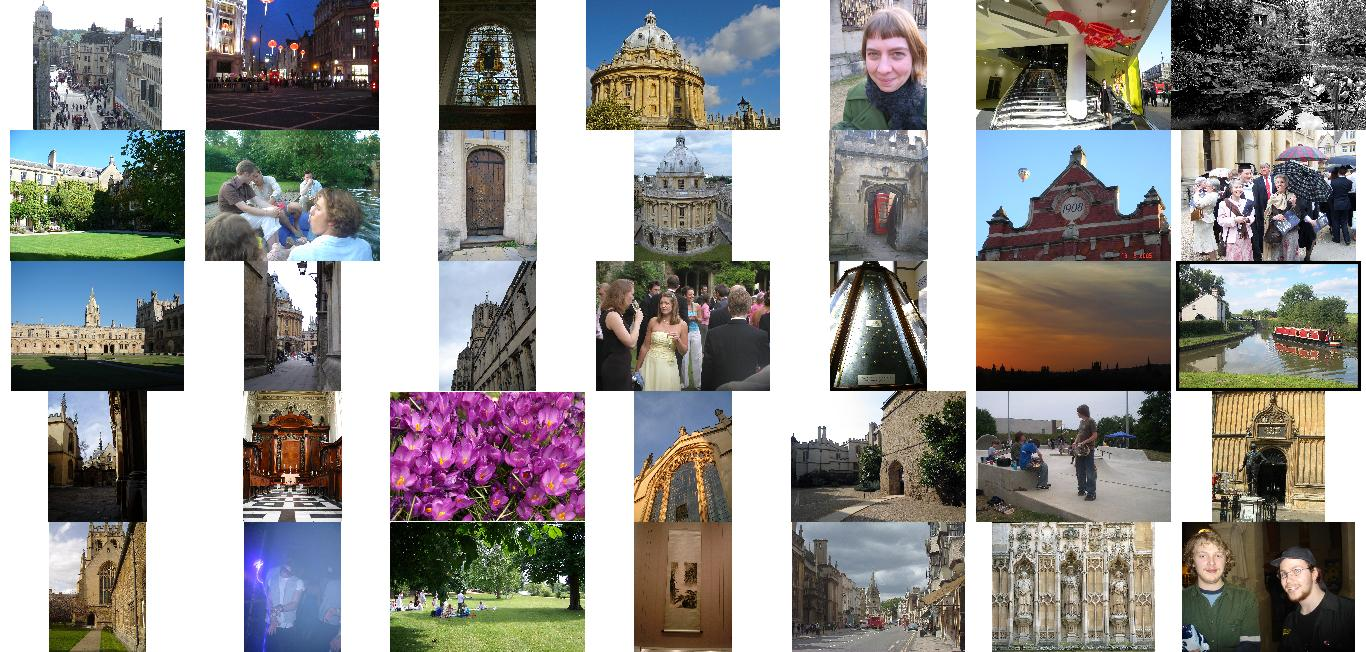
\includegraphics[width=3.0in]{oxbuilding.jpg}
    \caption{Some random images from Oxford Building 5K Dataset}
    \label{fig:oxbuilding}
\end{figure}

\begin{figure}
    \centering
    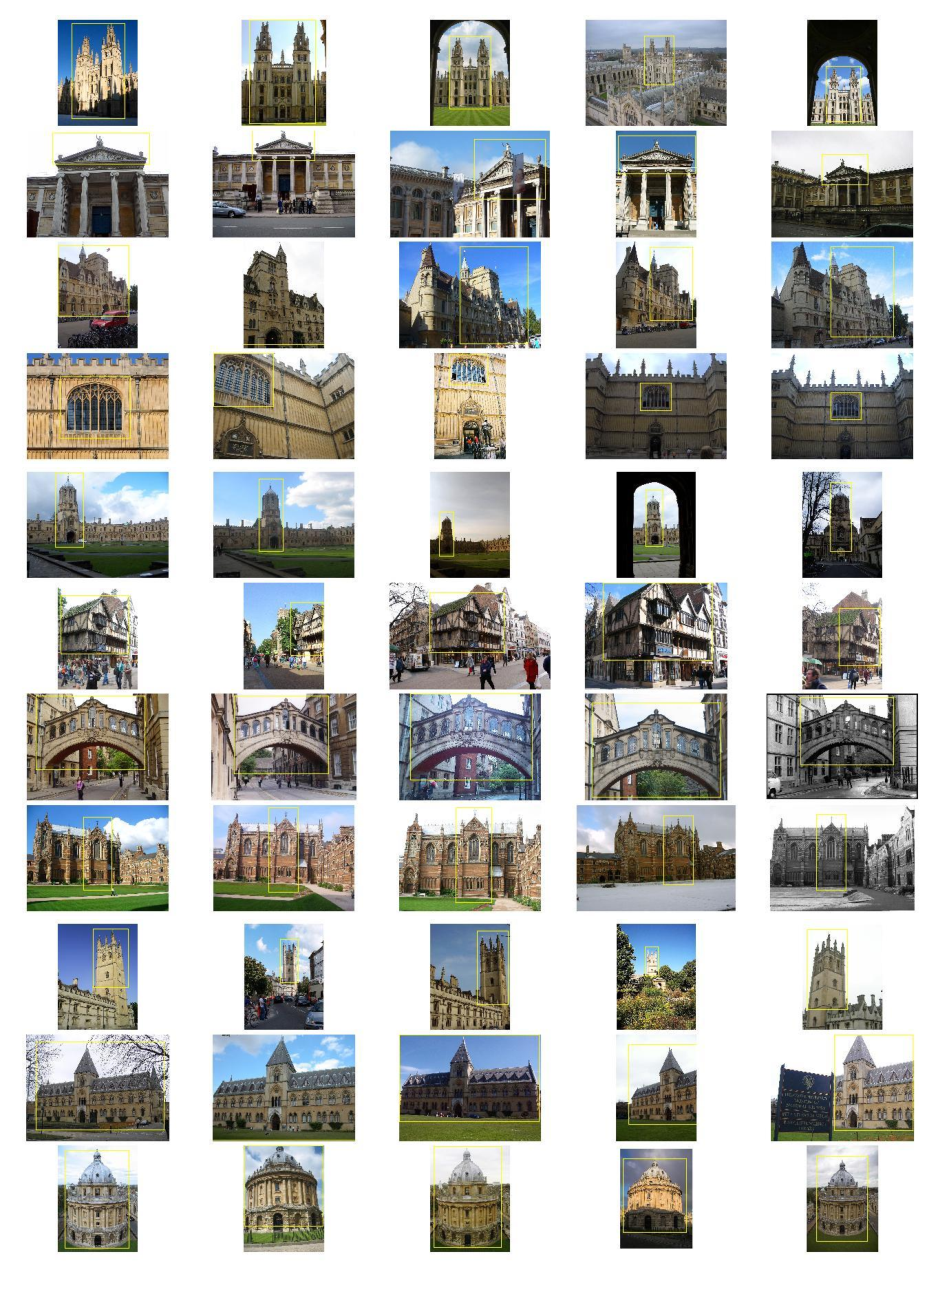
\includegraphics[width=3.0in]{oxbuilding_query.pdf}
    \caption{55 queries of Oxford Building 5K Dataset}
    \label{fig:oxbuilding_query}
\end{figure}

Our experiment shows that spatial rerank has significant impact on the retrieval quality of BoW model, an increase from 0.676 to 0.741 in term of mAP. More specifically, 74.2\% of the queries' AP are improved, the largest increment is from 0.417 to 1.000, the rest of queries approximately remain unchanged. The AP of all 55 queries are shown in figure \cite{fig:ap_chart}.

\begin{figure}
    \centering
    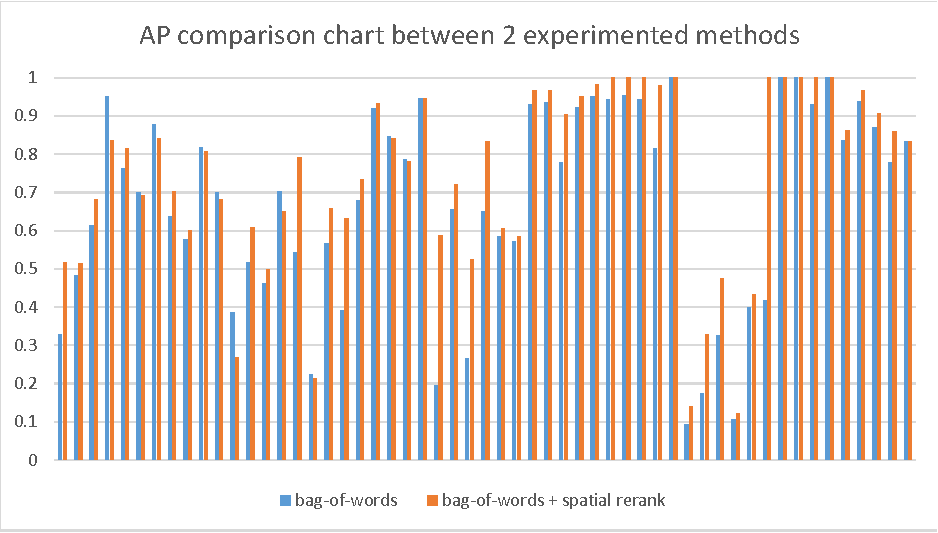
\includegraphics[width=3.0in]{mAP.pdf}
    \caption{Comparison chart between the 2 methods}
    \label{fig:ap_chart}
\end{figure}
